\begin{figure}
  \centering
  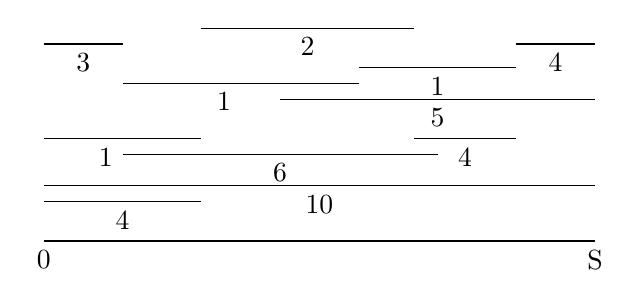
\begin{tikzpicture}
    \node at (0,0) [below] {0};
    \node at (7,0) [below] {S};

    \draw (2,2.7) -- node[below] {2} (4.7,2.7);
    \draw (0,2.5) -- node[below] {3} (1,2.5);
    \draw (6,2.5) -- node[below] {4} (7,2.5);
    \draw (4,2.2) -- node[below] {1} (6,2.2);
    \draw (1,2) -- node[below left] {1} (4,2);
    \draw (3,1.8) -- node[below] {5} (7,1.8);
    \draw (0,1.3) -- node[below left] {1} (2,1.3);
    \draw (4.7,1.3) -- node[below] {4} (6,1.3);
    \draw (1,1.1) -- node[below] {6} (5,1.1);
    \draw (0,.7) -- node[below] {10} (7,.7);
    \draw (0,.5) -- node[below] {4} (2,.5);
    \draw[thick] (0,0) -- (7,0);
  \end{tikzpicture}

  \caption{Ein Beispiel für das Grundstückproblem. Zahlen entsprechen den Profiten.}\label{fig:grundstueck}
\end{figure}